% Preamble
\documentclass[11pt]{article}
\usepackage[utf8]{inputenc}
\usepackage[T1]{fontenc}
\usepackage{amsmath,amssymb}
\usepackage{hyperref}
\usepackage{graphicx}

% Title
\title{Introduction to Elib's Monte Carlo Pricing Framework}
\author{Victor Felipe Gontijo}
\date{\today}

\begin{document}
\maketitle



\section{Overview}

Elib is a pricing library composed of three core modules:

\begin{enumerate}
  \item \textbf{Pricing Interface (Keops)}
  
    Elib exposes a C\# interface called \texttt{Keops}, used for setting up pricing requests and reading their corresponding results. A typical pricing request includes:
    \begin{itemize}
      \item a derivative product
      \item relevant market data
      \item a pricing model
      \item the desired mathematical quantities to be computed (price, Greeks, P\&L and lifecycle indicators, etc.)
    \end{itemize}

  \item \textbf{Product Script Module (OOPTA)}

    \texttt{OOPTA} provides a high-level, object-oriented ‘script’ representation of derivative products. This module defines systematic script layouts for equity derivatives, turning product descriptions into actual data structures. The latter are then used algorithmically throughout pricing computations during request execution.

    Intuitively, a derivative product defines a rule: for every "market trajectory" it produces a schedule of cash‐flows exchanged between issuer and holder.  
    Mathematically, the payoff of such a derivative product is a functional defined on the space of possible "market-paths". However, for exotic products, this functional might involve multiple conditions and it can be very hard to write explicitly.  
    
    The goal of a good script representation is to:
    \begin{itemize}
        \item Allow derivative products to be coded in a human-readable, financial-intuitive framework.
         \item Enable payoffs to be algorithmically evaluated without the need to manually translate the product’s term‐sheet features into complex explicit formulas.
    \end{itemize}
      
    Currently, OOPTA implements different script layouts, forming a set of \emph{Script Language Interfaces} (SLIs).  Each SLI is given by an abstract C\# class in OOPTA.  Thus, an actual product script corresponds to a class that derives the abstract logic from some pre-existing OOPTA SLI. This way, the generic logic is provided by the SLI, while particular custom features are added in the scripts' own specialized implementation.

  \item \textbf{Algorithmic Core (C++ Elib kernel)}

     Given a Keops request and an OOPTA script, an Elib pricing engine executes all computations to produce the requested outputs. 
       
     The set of pricing engines forms the algorithmic core of Elib. These are implemented in a C++ kernel, where performance considerations drive all development. Essentially, each engine applies a specific numerical method (analytic formulas, numeric PDE solvers, Monte Carlo estimators) to a particular pricing model to compute the requested quantities of a pricing request.

     In terms of software architecture, the Keops interface is responsible for piloting  
     the pricing workflow, while actual calculations are performed by the C++ Elib kernel.
     This is done through a series of callbacks and shared-memory buffers, passed between the three components. 
\end{enumerate}


\section{Keops Orchestration of Elib’s Pricing Workflow}

In this section, we describe the end-to-end Keops coordination of Elib’s Monte Carlo pricing routines.  We focus on the interplay between the three core components introduced earlier:

\subsection{Setting Up and Executing Pricing Command in Keops}
All begins by constructing a \texttt{Container} (\texttt{KeopsDomain}) object in Keops.  This container holds every entity needed to fully specify a pricing command:
\begin{itemize}
  \item Desired output quantities (price, Greeks, P\&L and lifecycle indicators)
  \item Product parameters (fixings, maturity, underlying assets' names)
  \item Product script (derived from some existing OOPTA SLI)
  \item Pricing model (reference to a model already coded in Elib)
  \item Market data (vol surfaces, historical price series, etc)
  \item Numerical algorithm (analytic formula, numerical PDE, Monte Carlo simulations).
\end{itemize}

The \texttt{Container} itself is just a dictionary of values—it does not execute any logic.  Once populated, Keops constructs a \texttt{PricingCommandRawData} object and triggers the pricing engine by calling: 
\begin{center}
    \begin{verbatim}
        command.GetService<ICommand>().Execute()
    \end{verbatim}
\end{center}
Essentially, the function call above dispatches the pricing command parameters into a true pricing routine, whose generic execution logic is implemented by the abstract C\# class \texttt{PricingEngineBase}.

\subsection{The "Textual Monte Carlo" setup}

We now restrict our focus to requests that activate the “Textual Monte Carlo” workflow.  In this case, the \texttt{PricingCommandRawData} object must include:

\begin{itemize}
  \item A \texttt{PricingAlgorithm} member of \texttt{MonteCarloAlgorithm} type.
  \item A \texttt{TradableToPrice} member of \texttt{TextualOption} type.
  The latter contains a product script written in one of the OOPTA SLIs that are compatible with Elib's Monte Carlo algorithm - We will focus on the most modern one, named \texttt{ContractPayoff}.
\end{itemize}

When Execute() is invoked, \texttt{PricingEngineBase} is specialized to the Keops class \texttt{TextualOptionMonteCarloPricer}.  In the next subsection, we examine how the latter overrides the method \texttt{PricingEngineBase::ComputeResults}.

\subsection{Launching the Monte Carlo Pricer}

Before entering the method \texttt{ComputeResults}, note that Keops uses the \texttt{ElibObject} wrapper to allocate and manage objects in unmanaged C++ memory.  This enables seamless callbacks into the C++ Elib kernel for high-performance routines.


Inside \texttt{TextualOptionMonteCarloPricer::ComputeResults}, three core \texttt{ElibObject} instances are created:

\begin{enumerate}
  \item \texttt{var product    = CreateProduct(...)}  
  \item \texttt{var transition = CreateTransition(...)}  
  \item \texttt{var pricer     = CreatePricer(..., product, transition, ...)}  
\end{enumerate}

These objects—\texttt{product}, \texttt{transition} and \texttt{pricer}—form the backbone of Elib’s Monte Carlo algorithm.  Once they are allocated and initialized in C++, the final pricing call is made:
\begin{verbatim}
  var res = Price(..., pricer, ...);
\end{verbatim}
This returns a \texttt{Tuple<ElibParam, ElibResults>}, also represented as \texttt{ElibObject} instances in C++ memory.  Upon exit, Keops marshals these results back into its own structures, making them available to the C\# client.

\section{Core C++ objects in the Monte Carlo algorithm}

As mentioned in the previous section, Elib’s Monte Carlo engine is built around three unmanaged C++ objects: the Product, the Transition and the Pricer. Each object has a well-defined role in the global process of initializing, simulating and evaluating paths.

\subsection{Product Object (\texttt{cal\_MC\_Product\_Textual})}
This class translates an OOPTA script into an unmanaged C++ product instance. Its constructor invokes OOPTA callbacks to parse the script and register each feature as a member variable. When the script implements the \texttt{ContractPayoff} SLI, the concrete C++ type instantiated is \texttt{MCTextualDescribedProduct}.


\subsection{Transition Object (\texttt{cal\_MC\_Transition})}
Encapsulates all logic for generating random market trajectories:
\begin{itemize}
  \item Configures the simulation time grid and discretization scheme.
  \item Initializes the basic risk-factors (Brownian increments), together with the volatility and correlation generators.
  \item Advances the modeled stochastic processes according to the model's evolution equation.
\end{itemize}

Each pricing model implements a specific derived "transition", which specializes the
mechanism for the generation of random market trajectories taking into account its own particular features.

\subsection{Pricer Object (\texttt{cal\_MC\_Generic\_Pricer})}
The \texttt{Pricer} coordinates the interaction of the product's \texttt{Product} and \texttt{Transition} objects. By doing so, it ensures Elib's Monte Carlo algorithm is able to:

\begin{enumerate}
    \item Initialize and launch per-thread pseudo-random generators for each risk factor.

    \item Simulate a block of market trajectories using the \texttt{Transition} object.
    
    \item Evaluate the payoff on each path via the \texttt{Product} object and aggregate statistics.
\end{enumerate}


\section{C++ Monte Carlo Execution Workflow}

As explained in the previous sections, Keops first initializes the three core C++ objects—\texttt{Product}, \texttt{Transition}, and \texttt{Pricer}—then calls:
\begin{verbatim}
  var res = Price(..., pricer, ...);
\end{verbatim}
This dispatches into the unmanaged kernel function
\verb|Elib_MCPricer_Price| (in namespace \texttt{PricingAlgorithm::MonteCarlo}), which launches the following call stack:

\begin{verbatim}
ElibMC_Pricer_Price
-> MetaPricer::computeScenarii
  -> MC_Generic_Pricer::price
    -> MC_Solver::Price_Portfolio
      -> MC_Solver::Loop
        -> MC_Solver::SimulateOnce
\end{verbatim}

\subsection{Vectorized Dispatch (\texttt{MetaPricer::computeScenarii})}
The \texttt{MetaPricer} decomposes the overall pricing task into multiple “simple” Monte Carlo runs—one per \emph{pricing context} (central and any bumped contexts). In code, this vectorized dispatch occurs in:

\begin{verbatim}
Elib_MCPricer_Price -> MetaPricer::computeScenarii
\end{verbatim}

For each context, it calls \texttt{MC\_Generic\_Pricer::price}, then aggregates all outputs into a single \texttt{PricingResultsWithGreeks} object.


\subsection{Core Monte Carlo Routine (\texttt{MC\_Generic\_Pricer::price})}

Within \texttt{MC\_Generic\_Pricer::price}, control is immediately passed to the private member \texttt{m\_MC\_Solver}, an instance of \texttt{MC\_Solver}.  This class forms the top layer of Elib’s Monte Carlo abstraction, directly orchestrating:

\begin{itemize}
  \item Pseudo-random number generation  
  \item Market-trajectory construction  
  \item Product payoff evaluations  
  \item Aggregation of pathwise statistics (e.g., pathwise Greeks, moments)  
\end{itemize}

Inside the \texttt{MC\_Generic\_Pricer::price} call, the \texttt{MC\_Solver} object carries out the MC algorithm is essentially by executing its following methods:

\begin{enumerate}
    \item \texttt{MC\_Solver::SetDesiredNumberOfTasks}: 
    Divides the total number of paths into thread-safe chunks, setting up work partitions for parallel execution of the future MC calculations.
        
    \item \texttt{MC\_Solver::setGenerator}: For each thread, constructs a \texttt{PerThreadData} object that encapsulates thread-local data, for each chunk of simulated paths.

    \item \texttt{MC\_Solver::Price\_Portfolio}: Launches the \texttt{Loop} method concurrently on all threads. Each thread accumulates its partial results into its corresponding \texttt{PerThreadData} object. Thus, thread-safety is ensured by forcing each thread to read and write in a separate memory location. 

\end{enumerate}

\subsection{Sequential Monte Carlo Loop (\texttt{MC\_Solver::Loop})}

\texttt{MC\_Solver::Loop} orchestrates each thread’s simulation cycle by processing fixed‐size blocks of 64 trajectories for SIMD efficiency.  Each loop iteration comprises two phases:

\begin{enumerate}
  \item \textbf{Generate basic random inputs for the new subblock of 64 random trajectories}
    \begin{itemize}
        \item Reloads the thread’s local buffer \texttt{perThreadData.m\_aleas} with fresh uniform variates via:
        \begin{verbatim}
        perthreadData -> GenerateAleasAndMeasureWeight(...)
        \end{verbatim}
       which selects the appropriate \texttt{MC\_AleasGenerator} and invokes  
    \texttt{getUniforms()} to fill 64 random vectors (each containing multiple uniform samples).
    \end{itemize}
      

  \item \textbf{Simulate 64 new trajectories and evaluate 64 payoffs (\texttt{SimulateOnce}).}
    \begin{itemize}
      \item Constructs each of the 64 market trajectories according to the model’s discretization scheme.
      \item Evaluates the product payoff along each path, handling early-exercise or barrier features as needed.
      \item Records trajectory statistics (cash-flow payments, barrier breaches, continuation-values at intermediate dates).
    \end{itemize}
\end{enumerate}

\begin{figure}[h]
  \centering
  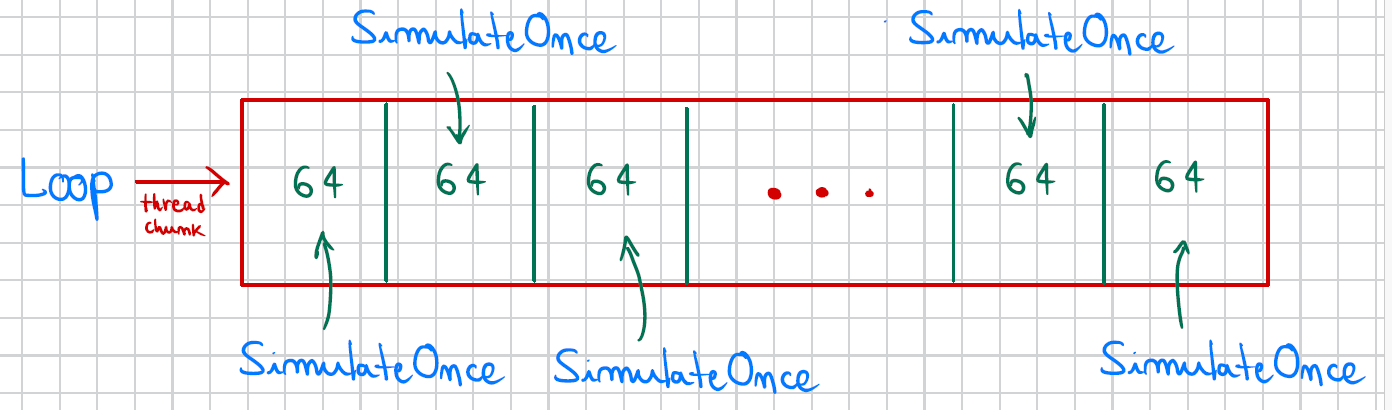
\includegraphics[width=\textwidth]{LoopScheme.png}
  \caption{Per‐thread processing in \texttt{MC\_Solver::Loop} - 64‐trajectory chunks are sequentially generated and payoff-evaluated by each internal call of \texttt{SimulateOnce}.}
\end{figure}

After all threads complete their \texttt{MC\_Solver::Loop} invocations, each thread has its own local empirical mean of discounted payoffs, \texttt{perThreadData.m\_PriceProductResult}. These local means are then merged into a global one - the price estimator - stored in the \texttt{Solver}’s global buffer \texttt{m\_Results}.


\subsection{Trajectory construction and Payoff evaluation (\texttt{MC\_Solver::SimulateOnce})} \label{construction-eval}

\begin{figure}[h]
  \centering
  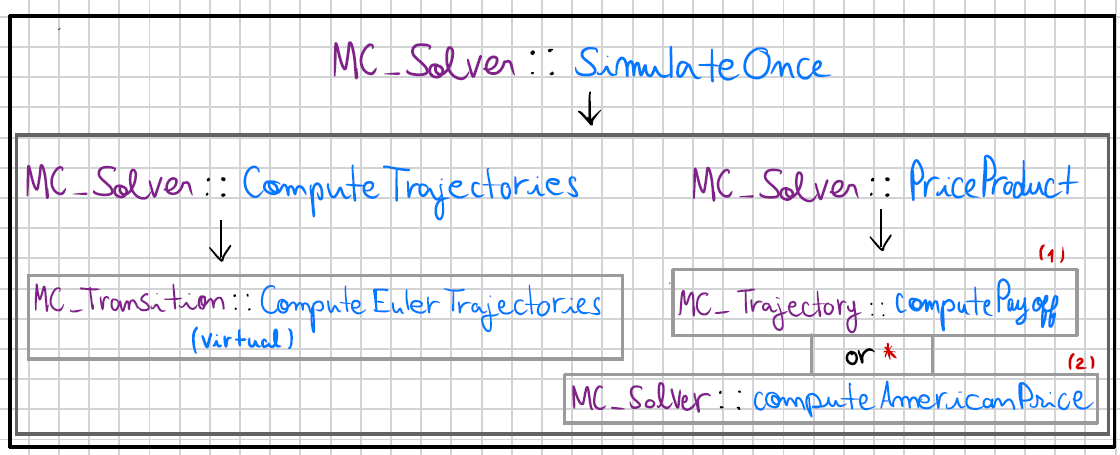
\includegraphics[width=\textwidth]{SimulateOnceScheme.png}
  \caption{Call flow within \texttt{MC\_Solver::SimulateOnce}: trajectories are built, then payoffs are computed.}
\end{figure}

Each call to \texttt{MC\_Solver::SimulateOnce} processes a sub‐block of 64 trajectories in two steps:

\begin{enumerate}
  \item (\textbf{Construct trajectories}): Invokes the virtual method  
    \begin{verbatim}
      MC_Transition::ComputeEulerTrajectories(...)
    \end{verbatim}
    
    to generate 64 paths according to the model’s discretization.
    This procedure relies on the input of 64 random vectors of uniform variables, stored in the thread’s local buffer \texttt{perThreadData.m\_aleas}.
    
    For Brownian‐motion models, these uniforms are converted into Brownian increments by the \texttt{m\_volGenerator} member of \texttt{MC\_Transition}.  Under the hood, \texttt{m\_volGenerator} holds an \texttt{IBrownianPathGenerator} instance that transforms a 2D array of uniforms into a multidimensional Brownian path.
    
  \item (\textbf{Evaluate payoffs}): Calls the method
  \begin{verbatim}
    MC_Solver::PriceProduct(...)
    \end{verbatim}
   which dispatches to either one of the following:
    \begin{itemize}
      \item \texttt{MC\_Trajectory::computePayoff(...)}, in the case of \texttt{Contract} SLI scripts.
      \item \texttt{MC\_Solver::computeAmericanPrice(...)}, , in the case of \texttt{ContractPayoff} SLI scripts.
    \end{itemize}
\end{enumerate}

Upon return from \texttt{PriceProduct}, the 64 resulting discounted payoffs are stored in the thread’s buffer vector \texttt{perThreadData.m\_PriceProductResult}. These values contribute to the thread’s local empirical mean, updated after each \texttt{MC\_Solver::SimulateOnce} call inside \texttt{MC\_Solver::Loop}.


\section{Payoff‐Modification Events and American Features}

Path‐dependent products — including options with early‐exercise or early‐termination features — pose two sources of randomness:
\begin{enumerate}
  \item The \emph{values} of cash‐flows.
  \item The \emph{timing} and \emph{existence} of those cash‐flows, which can depend on the simulated market path.
\end{enumerate}

\subsection{Tree Representation of Path‐Dependent Products}
To manage this complexity, Elib decomposes a path‐dependent product into a \emph{tree of simple contracts}, where each simple contract has a fixed schedule of cash‐flows (though their amounts remain random).  As a simulated trajectory “navigates” the tree, it may transition from one contract node to another whenever a payoff‐modification event occurs.

\begin{remark}
This tree view is natural in backward approaches to Bermudan option pricing and it naturally extends to the pricing of more general path-dependent options via terminal free-boundary PDEs.

The same “contract-tree” representation underpins finite-difference PDE methods: each node corresponds to a local free-boundary condition, and the backwards induction through the tree mirrors the backward time-stepping of the PDE.
\end{remark}

\subsection{Payoff‐Modification Events}
A \emph{payoff‐modification event} is any feature that can alter the remaining cash‐flow schedule in the mid‐life of the product.  Common examples include:
\begin{itemize}
  \item \textbf{Early exercise} (American/Bermudan options)  
  \item \textbf{Callable/puttable} triggers (issuer or holder termination rights)  
  \item \textbf{Barrier hits} (knock‐in/knock‐out)  
  \item \textbf{Conditional coupons} and \textbf{autocall} barriers  
\end{itemize}
At each observation date, Elib tests for applicable events and, if triggered, “shifts” the active contract node.

\subsection{Conditional Revaluation via Longstaff–Schwartz}
Some payoff-modification events can be checked using only backward‐looking information  (i.e they depend only on the history of the market trajectory up to the verification instant). On the other hand, other events require estimating the value of future cash flows (forward‐looking) given current market conditions, a process known as \emph{conditional revaluation}. 

For instance, conditional revaluation is required whenever we want to:
\begin{itemize}
    \item Determine the optimal early‐exercise or early‐termination policy at an intermediate date (exercise frontier determination)
    \item Regularize the product’s value profile immediately after a payoff‐modification event that introduces mathematical singularities (e.g. smoothing after a mid-life knock-out barrier) 
\end{itemize}

In the conditional revaluation process, the continuation value of the remaining cash flows is recomputed based on the prevailing market variables. To perform this estimation, Elib employs the Longstaff–Schwartz algorithm, which at each revaluation date proceeds through:

\begin{enumerate}
  \item \textbf{Continuation‐Value Approximation:}  
    Represent the continuation value as a conditional expectation and approximate it by a linear combination of preselected basis functions.  Elib evaluates these basis functions for each simulated path and stores the results in \newline \texttt{ValuesOnTrajectory::m\_decisionVariables}.

  \item \textbf{Coefficient Estimation via Regression:}  
    Simulate an independent batch of paths to maturity, recording the discounted future payoffs beyond the revaluation date.  Then perform a least‐squares regression of those payoffs onto the basis‐function values to obtain the regression weights.  These regressed coefficients complete the linear approximation of the continuation value.

    In code, \texttt{MC\_Solver::PriceProduct} calls:
    \begin{verbatim}
    MC_Solver::precomputeContinuationValuesRegressionMatrix(...)
    \end{verbatim}
    to compute the regression coefficients, instead of invoking \texttt{MC\_Solver::computeAmericanPrice} (which is used later during the payoff evaluation; see Section \ref{construction-eval}).
\end{enumerate}

\subsection{AmericanFeature Class and Data Structures}
Elib represents each payoff‐modification event as an instance of \texttt{AmericanFeature}.%
\footnote{The name “AmericanFeature” is a slight abuse of terminology, since “American” traditionally denotes optional early‐exercise, whereas payoff‐modification events also encompass non‐optional features (barriers, conditional coupons, etc.).}  Notable subclasses include:
\begin{itemize}
  \item \texttt{BarrierFeature}  
  \item \texttt{OptimalExercise}  
  \item \texttt{ContinuationValue}  
\end{itemize}
Each \texttt{AmericanFeature} instance holds:
\begin{itemize}
  \item An \emph{observation date}.  
  \item \texttt{m\_referenceContracts}: Contracts that can trigger this feature.  
  \item \texttt{m\_involvedContracts}: Contracts to which a trajectory may shift.  
  \item \texttt{m\_ValuesOnTrajectory}: Per‐trajectory quantitative data for checking event triggering path-wise (e.g., regression variables, barrier‐hit flags).
\end{itemize}

During each call of \texttt{MC\_Solver::SimulateOnce}, the member \texttt{m\_ValuesOnTrajectory} is refreshed for all 64 trajectories. When a product contains non‐trivial \texttt{AmericanFeature}s, payoff evaluation may require summing cash flows across multiple contract nodes. This logic is implemented in \texttt{MC\_Solver::computeAmericanPrice}, specifically within \texttt{MC\_Solver::computeAmericanLevel}.

Within that routine, each trajectory “traverses” the contract tree, encountering and processing relevant \texttt{AmericanFeature}s. After an event is applied, the active contract node is updated and subsequent cash flows are recorded accordingly.

\paragraph{Note on \texttt{ContinuationValue}:}  
Do not confuse the class \texttt{ContinuationValue} (derived from \texttt{AmericanFeature}) with \texttt{DRVContinuationValue} (derived from \texttt{DoubleRandomVariable}).  The relation between the two is that
the DRV object contains an instance of the former - the
member \texttt{m\_continuationValue}.


\section{Particularities of the PRIIPs Integration Developments}

\subsection{PRIIPs Transition}

The PRIIPs model uses a custom transition rather than the standard Brownian Euler scheme.  In the PRIIPs particular setting, we have:

\begin{itemize}
  \item \textbf{Integer‐valued alea generation.}  
    The array \texttt{perThreadData.m\_aleas} is originally populated by 
    \texttt{MC\_AleasGenerator::getUniforms()}, yielding 64 vectors of \([0,1]\)‐valued uniforms. In the PRIIPs transition, these uniforms are converted into integer indices (e.g.\ day‐offsets) by simple scalar multiplication and floor/cap operations. This conversion takes place in the method  \texttt{PriipsTrajectoriesGenerator::generatePastDatesShuffling}.

  \item \textbf{Trajectory construction on a coarse time mesh.}  
    Rather than generating a full daily‐price time-mesh, we can work with a coarser time-mesh and store increments over larger units of time. To do so, we need to sum
    over intermediate daily log‐returns, but we don't need to store them once the sum is calculated. This is what is actually implemented in the method \texttt{PriipsTrajectoriesGenerator::generateMultiAssetLogPricePaths}. The scheme below illustrates the relation between the different variables in the function:

     \begin{figure}[h]
      \centering
      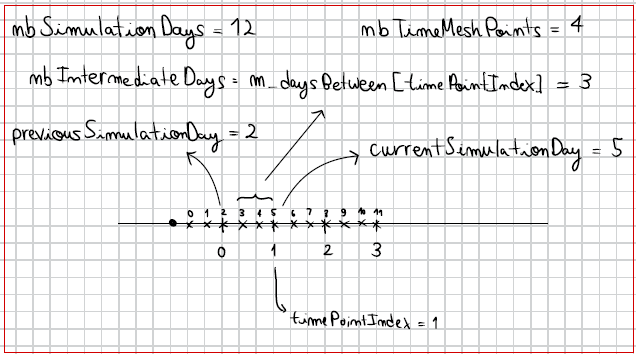
\includegraphics[width=\textwidth]{PriipsTimeMeshScheme.png}
      \caption{Coarse time-mesh mapping in generateMultiAssetLogPricePaths}
\end{figure}
\end{itemize}

%\subsection{Drift-bumped contexts}


\subsection{Empirical Distributions}

To capture the full empirical distribution of path‐functionals at various dates, Elib introduces the \texttt{EmpiricalDistribution} class. This utility collects observations incrementally during the Monte Carlo run, in a thread-safe manner.

In the PRIIPs project, we use \texttt{EmpiricalDistribution} instances to track two quantities, and in both cases, observations are computed and recorded during the execution of \texttt{MC\_Solver::computeAmericanLevel}:

\begin{enumerate}
  \item \textbf{Final Discounted Payoffs:}  
    The discounted terminal payoffs in the central pricing scenario are recorded directly by the solver via  
    \begin{verbatim}
MC_Solver::storeNewBlockOfDiscountedPayoffEvals(...)
    \end{verbatim}

  \item \textbf{Intermediate Holder PnL:}  
    In a drift‐bumped context, we track the capitalized P\&L of the holder.  An \texttt{Indicator} instance — containing specifically a \texttt{DRVHolderPnL} member —computes each path’s P\&L and feeds these values into the corresponding \texttt{EmpiricalDistribution}. 
    
    Unlike most Elib \texttt{Indicator}s, which are defined in the \texttt{Product} script, these PRIIPs PnL indicators are injected during OOPTA compilation of \texttt{ContractPayoff} scripts by:  
    \begin{verbatim}
    ContractPayoff.AddPriipsPerformanceIndicators(...)
    \end{verbatim}
\end{enumerate}


\end{document}
